% This is the Reed College LaTeX thesis template. Most of the work 
% for the document class was done by Sam Noble (SN), as well as this
% template. Later comments etc. by Ben Salzberg (BTS). Additional
% restructuring and APA support by Jess Youngberg (JY).
% Your comments and suggestions are more than welcome; please email
% them to cus@reed.edu
%
% See http://web.reed.edu/cis/help/latex.html for help. There are a 
% great bunch of help pages there, with notes on
% getting started, bibtex, etc. Go there and read it if you're not
% already familiar with LaTeX.
%
% Any line that starts with a percent symbol is a comment. 
% They won't show up in the document, and are useful for notes 
% to yourself and explaining commands. 
% Commenting also removes a line from the document; 
% very handy for troubleshooting problems. -BTS

% As far as I know, this follows the requirements laid out in 
% the 2002-2003 Senior Handbook. Ask a librarian to check the 
% document before binding. -SN

%%
%% Preamble
%%
% \documentclass{<something>} must begin each LaTeX document
\documentclass[12pt,twoside]{reedthesis}
% Packages are extensions to the basic LaTeX functions. Whatever you
% want to typeset, there is probably a package out there for it.
% Chemistry (chemtex), screenplays, you name it.
% Check out CTAN to see: http://www.ctan.org/
%%
\usepackage{graphicx,latexsym} 
\usepackage{amssymb,amsthm,amsmath}
\usepackage{longtable,booktabs,setspace} 
\usepackage{chemarr} %% Useful for one reaction arrow, useless if you're not a chem major
\usepackage[hyphens]{url}
\usepackage{rotating}
\usepackage{natbib}
\usepackage[utf8]{inputenc}

% Packages added by Me
%###############################
\usepackage{epigraph}
\usepackage{mathdesign}
\usepackage[hang, flushmargin]{footmisc}
%###############################

% Comment out the natbib line above and uncomment the following two lines to use the new 
% biblatex-chicago style, for Chicago A. Also make some changes at the end where the 
% bibliography is included. 
%\usepackage{biblatex-chicago}
%\bibliography{thesis}

% \usepackage{times} % other fonts are available like times, bookman, charter, palatino

\title{Mommy Fishues}
\author{Marissa Breanne Borrego}
% The month and year that you submit your FINAL draft TO THE LIBRARY (May or December)
\date{May 2019}
%\division{Mathematics and Natural Sciences}
\advisor{Suzy C. P. Renn}
%If you have two advisors for some reason, you can use the following
%\altadvisor{Your Other Advisor}
%%% Remember to use the correct department!
\department{Neuroscience}
% if you're writing a thesis in an interdisciplinary major,
% uncomment the line below and change the text as appropriate.
% check the Senior Handbook if unsure.
\thedivisionof{The Established Interdisciplinary Committee for Neuroscience}
% if you want the approval page to say "Approved for the Committee",
% uncomment the next line
\approvedforthe{Committee}

\setlength{\parskip}{0pt}
%%
%% End Preamble
%%
%% The fun begins:
\begin{document}

  \maketitle
  \frontmatter % this stuff will be roman-numbered
  \pagestyle{empty} % this removes page numbers from the frontmatter

% Acknowledgements (Acceptable American spelling) are optional
% So are Acknowledgments (proper English spelling)
    \chapter*{Acknowledgements}
	\epigraph{Any situation in which some individuals prevent others from engaging in the process of inquiry is one of violence.}{\textit{Paulo Freire \\ Pedagogy of the Oppressed}}
	
	I have been so very privileged to have the experience of attending college and writing a thesis. Any success I have had has been based in my access to extracurriculars, present parents, and supportive friends. I would like to thank:
	
	Suzy for pushing me to take the thesis process into my own hands and not giving up on me when I was having an incredibly hard time at the beginning of the year.
	
	Paul for mentoring me throughout my undergraduate experience and giving me so many opportunities to learn. I must thank you for teaching me to be critical of how science is done.
	
	Larry for supporting me in my research and giving me so much encouragement and so many resources. It has been such a wonderful experience to work at ONPRC.
	
	Presence for listening to all of my complaints, anxieties, and fears; for letting me curl up in a ball on the floor; for being a friend and mentor; for encouraging me to challenge the systems I am a part of; for introducing me to Pixie, Pax, and Noah; for so much more.
	
	James for helping me through the hardest part of my life, for inspiring me to study neuroscience, for giving me endless love and support.
	
	Langston for supporting my curiosities in math, programming, queerness, love, pretentious Portland stereotypes, etc.
	
	Duncan for opening your arms after every time I ignored your advice and then regretted doing so. You are such a strong being.
	
	Cam for being a great friend, an absent roommate, an incredible scientist, and perhaps most importantly, a truly interesting person.
	

% The preface is optional
% To remove it, comment it out or delete it.
    \chapter*{Preface}
	Science has a history as an oppressive institution. That being said, I think that science has the ability to liberate individuals through challenging the notion of self determination. I hope that this thesis is found to be accessible and at least makes one think of how plastic we are to our day-to-day experiences.

    \chapter*{List of Abbreviations}

	\begin{table}[h]
	\centering % You could remove this to move table to the left
	\begin{tabular}{ll}
    \textbf{11$\beta$-HSD2} & 11$\beta$-hydroxysteroid dehydrogenase type 2\\
    \textbf{ACTH} & Adrenocorticotropin hormone\\
    \textbf{CRH} & Corticotropin-releasing hormone \\
    \textbf{CPP} & Conditioned place preference\\
    \textbf{GR} & Glucocorticoid receptor \\
    \textbf{GRE} & Glucocorticoid response element \\
    \textbf{HLG} & High licking \& grooming \\
    \textbf{HPA} & Hypothalamic-pituitary-adrenal \\
    \textbf{LLG}  	&  Low licking \& grooming \\
    \textbf{PCR} & Polymerase chain reaction\\
    \textbf{PVN} & Pareventricular nucleus \\
    \textbf{qPCR} & Quantitative polymerase chain reaction\\
	\end{tabular}
	\end{table}
	

    \tableofcontents
% if you want a list of tables, optional
    \listoftables
% if you want a list of figures, also optional
    \listoffigures

% The abstract is not required if you're writing a creative thesis (but aren't they all?)
% If your abstract is longer than a page, there may be a formatting issue.
    \chapter*{Abstract}
	The preface pretty much says it all.
	
	\chapter*{Dedication}
  \epigraph{And in our hearts\\ How beautiful the flames that will flare up in a
    ring}{Chika Sigawa \\ ``Mountain Range''}
For Langston.
  \mainmatter % here the regular arabic numbering starts
  \pagestyle{fancyplain} % turns page numbering back on

%The \introduction command is provided as a convenience.
%if you want special chapter formatting, you'll probably want to avoid using it altogether

    \chapter*{Introduction}
         \addcontentsline{toc}{chapter}{Introduction}
	\chaptermark{Introduction}
	\markboth{Introduction}{Introduction}
	% The three lines above are to make sure that the headers are right, that the intro gets included in the table of contents, and that it doesn't get numbered 1 so that chapter one is 1.

% Double spacing: if you want to double space, or one and a half 
% space, uncomment one of the following lines. You can go back to 
% single spacing with the \singlespacing command.
% \onehalfspacing
% \doublespacing
		
A defining feature of living organisms is that they are able to respond to
stimuli in their environment. In other words, they behave. Each behavior
requires an external stimulus, or multiple stimuli, that triggers a chain
reaction of internal responses, changing how an organism exists in its environment. In understanding why an animal responds to a stimulus in the way it does, there
are two places to start. One can look to the organism's genotype \textit{i.e.},
was this behavior inherited genetically from its parents? Or one can look to the
organism's upbringing \textit{i.e.}, was this behavior learned in response to
the enviornment, over the course. Traditionally, these two possibilities have been thought of as
separate and exclusive, as in the phrase \textit{nature} vs \textit{nurture}.  

The dichotomy of nature and nurture as we know it today has its unfortunate beginnings in
the field of eugenics. The phrase was popularized by the father of eugenics, Francis
Galton, in the late 19th century in an effort to understand if human ``ability''
was heritable. He defined nature as ``all that a man brings with himself into
the world'' and nurture as ``every influence from without that affects him after
his birth.'' (Galton, 1874) While there was not yet a concept of DNA, both
Darwin's theory of evolution and Mendel's inheritence experiments were in
circulation. The interest in nature \textit{vs} nurture remained within developmental
psychology until late in the 20th century when behavioral and developmental
neurosciences were popularized.

In the early and mid 20th century, the fields of animal behavior and
genetics were being revolutionized in ways that would ultimately contribute to the modern debate of
nature and nurture (Krubitzer \& Kahn, 2003). In the 1930's a pioneering behavioral scientist by the name of Nikolaas Tinbergen began
studying behaviors holistically, as a product of individual
experience and evolution. He was interested in creating a scientifically
rigorous way by which to observe and comment on behavior.
What emerged was the modern field of ethology and a set of four categories to
study a behavior through: causation (mechanism), survival value (adaptation),
ontogeny, and evolution (Tinbergen, 1963).
Tinbergen's four questions were important in examining a single behavior as a product of an
individual's experiences and that individual's lineage. That being said, there
was still a gap in understanding how molecular biology contributed to all of this.

Abstract concepts of DNA and RNA as a heritable molecule had been proposed by the early 20th century in response to heritability
studies (Koltzoff, 1934; Hershey \& Chase, 1952), but it wasn't until
Francis Crick and James Watson published a study in 1953 on the structure of DNA
(notably, the 
study relied heavily on prior work by Rosalind Franklin) that
the field of modern genetics really began (Watson \& Crick, 1953). Using
information about base pairs and amino acids published by other labs at the
time, in 1955 Crick proposed the
central dogma of genetics. This crucial concept states that DNA is translated into RNA, which is then
transcribed into amino acids that are linked together to form proteins.

The last big step in getting to our current concept of nature and nurture was
the popularization of epigenetics. Epigenetics, in short (this concept will be
more deeply explored in Chapter 1), refers to
the factors that change the ability of DNA to be transcribed, contributing to
changes in gene expression. Much of modern behavioral sciences is aimed at understanding
how the environment influences an organisms epigenome. 

Because we now understand gene expression is often altered by the environment, our notion of
nature \textit{vs} nurture becomes rather arbitrary. Behaviors can instead be
thought of as an intertwining of nature \textit{and} nurture. Rather than
understanding the ratio of environmental to genetic influence on a behavior, we
can instead examine how certain genotypes make an organism more vulnerable to
environmental influences or how the environment influences the quantity of a
protein produced. 

Put simply, this thesis will examine how maternal care (a stimulus) affects
stress response (a behavior) in a mouth-brooding fish. I will begin by
explaining epigenetics and physiological components of the stress response. Then
I will give a brief summary of what is already known about maternal care's
influence on behavior, before diving into the novel research I conducted. I will
conclude with the implications of my study and future directions for this
line of research.

%\chapter{Nature vs Nurture: Another Binary that Doesn't Exist}



%An organism's genotype is capable of influencing how it responds to its
%environment. Take for example the idea of \textit{genetic risk factors}. These
%are alleles that predispose an individual to being affected by an
%environmental factor. A study by Klengel \textit{et al.}, found that the
%occurence of PTSD in people with a \textit{protective} FKBP5 allele was not
%influenced by their experience with childhood trauma. In contrast, people that
%experienced physical and sexual abuse with the \textit{risk} alleles were more
%than twice as likely to develop PTSD compared to their non-abused
%counterparts(PTSD paper). This finding challenges the idea that environment
%operates separately from genotype in producing a phenotype. It also alludes to a
%major theme of this thesis which is that early life experiences can contribute to
%life-long changes to the brain.

%\section{Epigenetics}

%As described in the introduction, epigenetics refers to `` the study of stable
%alterations in gene expression potential that arise during development and cell
%proliferation'' (Jaenisch \& Bird, 2003). Cells in the heart and brain have the
%same DNA, but it is differences in their gene expression that result in
%differences of morphology and function. To understand how genes become more or
%less likely to be transcribed, we must look to the structure of DNA. When DNA is
%not being copied (most of the time), it takes on a folded, condensed form called
%chromatin. As chomatin, the DNA is wound around proteins called
%histones. There are hundreds of ways that histones can be modified (Kouzarides,
%2007). These modifications can, for example, make chromatin less accessible to
%transcription proteins.

%Two common forms of epigenetic
%changes are histone modification and DNA methylation.  

\chapter{Stress, Epigentics, and Early-Life Experience}

\section{The Mechanisms of Stress}
If you have made it this far in life, you have at some times felt
\textit{stressed}. Stress can be
defined as the body's response to and recovery from a threat that disrupts
homeostatis (Bodegom). We often times think about stress negatively; however our
ability to respond to stressors is essential for our day-to-day lives. It is the
exposure to chronic levels of stress which disrupts our ability to live well.

\subsection{The Hypothalamic-Pituitary-Adrenal Axis}
 An important aspect of the stress response is the production and mobilization
 of energy. This is made possible through the hypothalamic-pituitary-adrenal (HPA)
axis because it functions to produce glucocorticoids. The activation of the HPA
axis in response to an immediate stressor occurs through stimulation by other brain areas, usually those involved in
homeostasis. For example, a painful stimulus may cause afferent signaling to
norepinephrinergic neurons in the hind brain, which in turn stimulate neurons in
the hypothalamus. It is also possible to activate the HPA axis as an
anticipatory response, which requires polysynaptic signaling from limbic
structures such as the hippocampus and amygdala. It is hypothesized that much of
the amygdalar signaling works through disinhibition, \textit{i.e.,} GABAergic interneurons
inhibit the GABAergic neurons that inhibit the HPA-axis. In contrast,
the hippocampus excites the axis through the use of glutamatergic interneurons.

The hypothalamus is a region of the midbrain known
for its role in maintaining allostasis through its involvement in stress,
appetite, circadian rhythms, and sexual behavior. In response to a stressor the
paraventricular nucleus (PVN) of the hypothalamus secretes
corticotropin-releasing hormone (CRH) and vasopressin, which bind to receptors
in the pituitary gland.

The pituitary gland is directly ventral to the hypothalamus and is a main
regulator of hormone release. The binding of CRH to CRH R1 receptors in the
anterior pituitary leads to the secretion of adrenocorticotropin hormone (ACTH).
This excitatory interaction can be potentiated by vasopressin, though
vasopressin alone is not enough to produce an effect. 

ACTH enters the blood stream and travels to the adrenal cortices, which are the dorsal
regions of the adrenal glands. ACTH binds to melanocortin 2 receptors, which
increases the synthesis of cholesterol. Cholesterol is then transported to the
outer mitochondrial matrix where the steroidogenic pathway begins. One important
product of this pathway is corticosteroids, the major product of the HPA axis.

Corticosteroids are a class of steroid hormones that can bind to glucocorticoid receptors (GRs)
and mineralocorticoid receptors. GRs are found throughout
the brain, notably within the hypothalamus and pituitary where they play a negative
feedback role for the HPA axis. Additionally, GRs are found in prominant
forebrain structures, such as the hippocampus and prefrontal cortex. When
cortisol binds to a GR, the GR disassociates from the cellular membrane and is
transported to the nucleus where it dimerizes with another GR. The heterodimer
can then interact with other proteins, ultimately leading to the binding of the
complex to a glucocorticoid response element (GRE) on the genome. These GREs are often
found in the promotor region of their target genes. The GREs then recruit
transcription factors to suppress or enhance transcription of the target gene
(Tsai book, Herman).
Ligand binding to GRs can also have nongenomic consequences such as kinase
activation, though these pathways are not well understood.
(Samarasinghe, 2011).
%The G-coupled protein receptors, when activated,
%act as a transcription factor in the nuclear and mitochondrial genome, making
%them capabe of largely influencing the brain's epigenome (mito paper).

In mammals, there are eight known transcriptional isoforms of the GR gene (Saif,
2015) and
thirteen different post-translational modification sites of the GR (Oakley \&
Cidlowski, 2013), altering the
cellular function (Lu, Collins, Grissom, \& Cidlowski, 2007). A genome duplication event happened in the evolution of teleosts, causing them
to have two GR paralogues. Both GR1 and GR2 are expressed in corticosteroid
responsive regions,
suggesting that they both maintain signaling functionality. Furthermore, the gene sequences are
highly similar to each other as well as to GR genes of other species (Greenwood,
2003).

%%%%%%%%%%%%%%%%%%%%%%%%%%%%%%%%%%%%%%%%%%% More on actual mechanism, cause, and
%%%%%%%%%%%%%%%%%%%%%%%%%%%%%%%%%%%%%%%%%%% effect 

% Figure of HPA axis 
\subsection{The Stress Response Beyond HPA}

Triggering of the HPA-axis ends with the release of cortisteroids, which can
easily cross the blood-brain-barrier and have a number of forebrain targets.
Important is the influence that the initial stress response has on the limbic
system. The amygdala plays a role in anxiety and fear behavior and is known to
be a regulator of the HPA-axis.

\section{Chronic Stress}
The fact that chronic stress is often unhealthy is quite intuitive. When an
organism is forced to expend energy on immediate survival, it must forego less
pressing, but very important processes like eating, sleeping, reproducing, and
learning. The following section will examine some of the biological
underpinnings of the maladaptive nature of chronic stress.  


\subsection{The Effects of Prenatal Stress on Development}
Glucorticoids receptor play an important role in fetal development. While
insufficient levels of glucocorticoids are fatal, causing undeveloped lungs,
excess circulating glucorticoids are also maladaptive, leading to developmental
reprogramming (Tsai book). The offspring of pregnant mice treated with synthetic glucocorticoids
 have delayed maturation of neurons and glia as well as delayed vascularization
 of the brain (olabi). Further, prenatal stress exposure is correlated with
 decreased dendritic spine density in the cingulate gyrus and orbitofrontal
 cortex (Murmu, 2006). These data suggest that prenatal stress alters the
 physiology and connectome of the developing brain.

 The ability of offspring to learn and form memories is altered by prenatal
 stress exposure. Compared to controls, offspring of stressed mothers have decreased fear learning in a
 passive avoidance behavioral paradigm (Sofiabadi, 2018). Older rats have impaired spatial memory in the Y-maze and
 working memory in the radial arm maze when they were exposed to prenatal stress
 (Valleem 2009). Rats also display a corresponding
 decrease in CAMKII and CREB mRNA expression in the hippocampus (Sun). 

 Rats exposed to prenatal stress are also more susceptible to addictive behavior.
 Rats with mothers exposed to stress have increased nicotine condition placed
 preference (CPP) as well as increased dopamine D$_2$ receptor gene expression
 in nucleus accumbens (Said, 2015). Prenatal stress has also been shown to
 increase CPP after in response to benzodiazepines (Lakehayli, 2015), cocaine
 (Pastor 2018), and morphine (Vey, 2016) just to name a few.

 Lastly, prenatal stress is a predictor of psychiatric disease in adults.
 Rodents exposed to prenatal stress show increased anxiety, depressive, and
 schizophrenic-like behavior compared to offspring of non-stressed dams
 (Weinstock, 2016). 

\subsection{The Effects of Postnatal Stress on Development}

\subsection{Protection Against Early Life Stress} 

There exists a highly conserved protection against early life stress in both
mammals and teleosts. In both cases, mothers secrete 11$\beta$-hydroxysteroid
dehydrogenase type 2 (11$\beta$-HSD2) into the prenatal environment throughout
pregnancy. This hormone rapidly deactivates corticosteroids, effectively
inhibiting the stress response of embryos (Bodegom 2017, zebrafish 11BHSD2). As
newborns, there is a stress hyporesponsiveness period characterized by a
decrease in circulating ACTH and corticosteroids, as well as an overall decrease
in responsiveness to stressors (Bodegom 2017, trout shrp).

Importantly, both of these defenses can be altered by a highly stressful
environment. Repeated maternal exposure to stress decreases 11$\beta$-HSD2,
increasing prenatal corticosteroid exposure. Additionally maternal separation is
associated with a shortened stress hyporesponsiveness period in mammals (no
similar study has been done in fish). These findings suggest that the stress
response is plastic to early life experience. This is
evolutionarily favorible in that it allows the animal to adapt to its
environment. The match/mismatch hypothesis suggests that organisms experiencing
adversity early in life will most likely face similar levels of adversity later
in life and should adjust their stress response to reflect that. With this
hypothesis comes the idea that a mismatch in early environment and adult
environment would have adverse consequences for the organism (Gluckman, 2007). 

\section{The Effects of Early Life Stress on the HPA Axis}

\subsection{Maternal Care and Stress}
The lab of Michael Meaney has done years of groundbreaking work on how maternal
care alters the stress response in rats.  Rat mothers exhibit consistent differences in the time spent licking and grooming
their young during their first week of life (Meaney, big paper citation 28). This difference takes place during a critical period
of the rats neural development. As a result, pups reared by high licking and grooming
(HLG) mothers and low licking and grooming (LLG) mothers have distinct
phenotypes and epigenomes (Meaney epigenome).

In 1997, Meaney's lab examined how ciculating stress hormones differed in pups
reared by HLG and LLG mothers. (Meaney, gluc). HLG pups had reduced circulating levels of ACTH and
corticosterone in response to restraint stress. Additionally, HLG pups appeared
to have enhanced regulatory feedback in stressful situations, as they surpressed
ACTH to a greater extent after being pre-treated with corticosterone (the murine
equivalent of cortisol). HLG pups
also developed higher GR expression in the hippocampus as adults. In a
complementary study, the lab found a distinct behavioral phenotype between the
two groups (behavioral). Rats reared by HLG dams exhibited more exploratory
behavior, as measured by an open field paradigm, compared to those reared by LLG
dams. Additionally, LLG pups exhibited a longer latency to start of eating when
placed in a novel environment compared to HLG pups. One year later, Meaney cross-fostered pups from HLG and
LLG mothers. As a result, pups born to LLG dams, but reared by HLG dams had a
similar phenotype to those born to and reared by HLG dams (transgenerational). These findings
indicated that maternal care can influence offsprings' responses to stress as
adults.

In 2004, Meaney
published a paper on the epigenetics of the above discoveries (Meaney epigenome). He found that the
epigenetic state of the GR promoter gene was altered by maternal licking and
grooming. This difference in methylation state was contingent on the rearing,
not the biological, mother.  GR receptor methylation was decreased and
acetylation increased in HLG rats, consistent with earlier studies. Taken
together, Meaney's work demonstates that rats reared by LLG dams have a
hypersensitive stress response, characterized by increased circulating stress
hormones, decreased hippocampal GR receptors, and decreased exploratory
behavior. 

\textbf{Taborsky work}
Barbara Taborsky extended the work of Michael Meaney to social fish species.
Most of Taborsky's work is with \textit{N. pulcher}, a highly social cichlid species
that live in family units and collectively raise offspring. Immature fish help
to keep eggs clean and well-oxygenated while adults defend the eggs against
predators and conspecifics (Arnold 2010).

Much of Taborsky's work has focused on
how early life social experience affects social behavior and stress response in
adults. Fish were divided into three groups: those raised with adults and
immature helpers, those raised with just helpers, and those raised with neither
helpers nor adults. Taborsky found that \textit{N. pulcher} fry raised in the
absense of adults and helpers had decreased social competency, showing
energetically costly levels of aggression in territory disputes (Arnold 2010). Fish raised with only their siblings also had decreased whole-brain GR1
expression and CRH compared to those raised in the presence of adults or helpers
(Taborsky 2012). A follow-up study examining specific regions of the brain
showed that fry raised in the presence of adults and helpers had increased in
GR1 mRNA expression in the telencephalon. Additionally, the blocking of GRs in fry reared without adults and helpers resulted in more appropriate
levels of aggression, indicating that the social effects of different rearing
environments are mediated in part by GR. (Nyman, 2018). Lastly, fry raised in
the absence of adults and helpers displayed more neophobia in behavioral tests,
which is indicative of higher stress in new environments (Bannier et al., 2017). 

% Table of studies

\textbf{\textit{A. burtoni}}
 \textit{A. burtoni}, the focus of this
thesis, are also a highly social cichlid. In this species, mother's carry the
fertilized eggs in their mouths, fasting until the fry hatch. Once hatched, the
fry spend time both in the mother's mouth and freely swimming for an addition
two weeks.    

% Fish Pics

A very recent study by Taborsky examined...
\subsection{The Gap in Our Knowledge}

The work of Barbara Taborsky has demonstrated that social fish species are
plastic to their early life experience, showing changes in behavior and stress
hormone expression. Her work however, is more focused on the effect that social
environment has on social behavior. There is little known about how maternal
separation affects mouth brooding fish. The presence or absence of mouth
brooding is an interesting behavior to study because it effects both prenatal
and postnatal environment. This research is crucial to
understanding the evolution of neural plasticity in response to early life
experience. If there are similarities between fish and mammals, this would
suggest a highly conserved adaptation to stressful environments.

A recent thesis by Destiny...

\chapter{The Experiment}

\section{Methods}
\subsection{The Fish}

The parental generation of the focal juveniles originated from a wild-caught stock of \textit{A. burtoni} collected from Lake Tanganyika. Social groups containing males and females of the same generation were kept in DIMENSIONS tanks at a temperature of TEMP and a pH of PH. Each tank's bottom was covered in gravel and terra cotta pot pieces were placed in the tank to act as shelters and territory markers. Females were monitored for mouth brooding behavior and were randomly assigned to an experimental condition. All females were collected within the first three days of brooding.

In the unseparated condition, mothers were removed from their home tank, weighed, and measured. They were then placed in small tanks containing gravel and a piece of terra cotta pot. Mothers continued to brood their young until the fry were old enough to regularly leave their mother's mouth, at which point the mother was removed from the tank to prevent her from eating the fry. 

In the separated condition, mothers were weighed and measured and then the eggs
were removed from their mouths by gently pulling down their bottom
lips. The eggs were then placed in a flask within a tank containing gravel. Once
the eggs developed into freely moving fry, the flask was removed from the tank and a piece of terra cotta was added.

Behavioral testing began approximately 130 days after the brooding mothers were placed into experimental conditions. 

\subsection{Behavioral Tests}
Prior to behavioral testing, each brood was moved in their home cage to the
testing area. They were allowed to adjust to the lighting for 10 minutes. 

\textbf{Boldness Assay}\\
Boldness, or willingness to explore novel and open environments, is often used as a measure of stress. Animals that are stressed tend to freeze in place, seek cover, and avoid open spaces. Focal fish were placed in a novel aquarium containing gravel and a terra cotta shelter. They were allowed to acclimate for 10 minutes before their behavior was scored for another 10 minutes. Boldness was measured on three axes: time spent in top half of tank, time spent frozen, and time spent under the shelter. \\
\\
\noindent\textbf{Aggression Assay}\\
Because \textit{A. burtoni} are highly social fish, we were interested in how maternal separation would affect their social behavior. Individual broods were transferred into a novel aquarium containing only water. The fish were allowed to acclimate to the new environment for 10 minutes before scoring began. The number of charges, bites, and chases between fish that occurred in 10 minutes were recorded and divided by the number of fish in the brood to create a score. Broods that only had one fish in them were excluded from this paradigm.  

% Figure of experimental set up

\subsection{Gene Expression Assay}
Directly following behavioral testing, fish were measured and quickly euthanized
via decapitation. The brains were then extracted and placed into RNAlater, and
stored at 4 $^\circ$C. 
\begin{table}[htbp]
\caption[Genes and Corresponding Primers Used for qPCR]{Genes and Corresponding
  Primers Used for qPCR}
\begin{center}
\footnotesize
\begin{tabular}{ | c | c | c | c | c |}
\hline
Target & Forward & Reverse & T$_{m}$\\
\hline
gr2 & TGC CTC TGT CAC TGC CAC CGT AG & AGT CGT CTG CGT CTG AAG TAA CTG &  60.9  $^{\circ}$C\\
\hline
gr1a & TCA TAA GAT CTG TTT GGT GTG CTC & GTA GTT GTG CTG GCC TTC AAC &  \\
\hline
gr1b & TGT TGG CTT CTC CGG TTC ATC AC & GTT GTG CTG GCC ATC TGT GTT T &  60.9 $^{\circ}$C\\
\hline
rfl23 & TGC TGA TGC CCA ACA TCG GTT & TCT TGG AGG AGA CAT TGT GGG &  55.7  $^{\circ}$C\\
\hline
\end{tabular}
\end{center}
\end{table}
\textbf{Troubleshooting}
Prior to working with experimental fish, an age-matched brood was used to
troubleshoot behavioral testing. Following that, the brood was euthanized using
MS-22 to practice brain extractions. Two of the extracted brains were used for
gene expression troubleshooting. RNA was extracted from the brains and reverse
transcribed into cDNA. All of the primer sets were tested using PCR on a gradient of
melting temperature using this cDNA. The most effective melting temperature was
then selected for qPCR.
\section{Results}

\chapter{What Does this Mean?}

%\chapter{The Rest}
	
% \section{References, Labels, Custom Commands and Footnotes}
% It is easy to refer to anything within your document using the \texttt{label} and \texttt{ref} tags.  Labels must be unique and shouldn't use any odd characters; generally sticking to letters and numbers (no spaces) should be fine. Put the label on whatever you want to refer to, and put the reference where you want the reference. \LaTeX\ will keep track of the chapter, section, and figure or table numbers for you. 

% \subsection{References and Labels}
% Sometimes you'd like to refer to a table or figure, e.g. you can see in Figure \ref{subd2} that you can rotate figures . Start by labeling your figure or table with the label command (\verb=\label{labelvariable}=) below the caption (see the chapter on graphics and tables for examples). Then when you would like to refer to the table or figure, use the ref command (\verb=\ref{labelvariable}=). Make sure your label variables are unique; you can't have two elements named ``default." Also, since the reference command only puts the figure or table number, you will have to put  ``Table" or ``Figure" as appropriate, as seen in the following examples:

%  As I showed in Table \ref{inheritance} many factors can be assumed to follow from inheritance. Also see the Figure \ref{subd} for an illustration.
 
% \subsection{Custom Commands}\label{commands}
% Are you sick of writing the same complex equation or phrase over and over? 

% The custom commands should be placed in the preamble, or at least prior to the first usage of the command. The structure of the \verb=\newcommand= consists of the name of the new command in curly braces, the number of arguments to be made in square brackets and then, inside a new set of curly braces, the command(s) that make up the new command. The whole thing is sandwiched inside a larger set of curly braces. 

% % Note: you cannot use numbers in your commands!
% \newcommand{\hydro}{H$_2$SO$_4$}

% In other words, if you want to make a shorthand for H$_2$SO$_4$, which doesn't include an argument, you would write: \verb=\newcommand{\hydro}{H$_2$SO$_4$}= and then when you needed  to use the command you would type \verb=\hydro=. (sans verb and the equals sign brackets, if you're looking at the .tex version). For example: \hydro

% \subsection{Footnotes and Endnotes}
% 	You might want to footnote something.\footnote{footnote text} Be sure to leave no spaces between the word immediately preceding the footnote command and the command itself. The footnote will be in a smaller font and placed appropriately. Endnotes work in much the same way. More information can be found about both on the CUS site.
	
\section{Bibliographies}
	Of course you will need to cite things, and you will probably accumulate an armful of sources. This is why BibTeX was created. For more information about BibTeX and bibliographies, see our CUS site (\url{web.reed.edu/cis/help/latex/index.html})\footnote{\cite{reedweb:2007}}. There are three pages on this topic: {\it bibtex} (which talks about using BibTeX, at \url{/latex/bibtex.html}), {\it bibtexstyles} (about how to find and use the bibliography style that best suits your needs, at \url{/latex/bibtexstyles.html}) and {\it bibman} (which covers how to make and maintain a bibliography by hand, without BibTeX, at at \url{/latex/bibman.html}). The last page will not be useful unless you have only a few sources. There used to be APA stuff here, but we don't need it since I've fixed this with my apa-good natbib style file.
	
% \subsection{Tips for Bibliographies}
% \begin{enumerate}
% \item Like with thesis formatting, the sooner you start compiling your bibliography for something as large as thesis, the better. Typing in source after source is mind-numbing enough; do you really want to do it for hours on end in late April? Think of it as procrastination.
% \item The cite key (a citation's label) needs to be unique from the other entries.
% \item When you have more than one author or editor, you need to separate each author's name by the word ``and'' e.g.\\ \verb+Author = {Noble, Sam and Youngberg, Jessica},+.
% \item Bibliographies made using BibTeX (whether manually or using a manager) accept LaTeX markup, so you can italicize and add symbols as necessary.
% \item To force capitalization in an article title or where all lowercase is generally used, bracket the capital letter in curly braces.
% \item You can add a Reed Thesis citation\footnote{\cite{noble:2002}} option. The best way to do this is to use the phdthesis type of citation, and use the optional ``type'' field to enter ``Reed thesis'' or ``Undergraduate thesis''. Here's a test of Chicago, showing the second cite in a row\footnote{\cite{noble:2002}} being different. Also the second time not in a row\footnote{\cite{reedweb:2007}} should be different. Of course in other styles they'll all look the same.
% \end{enumerate}
% \section{Anything else?}
% If you'd like to see examples of other things in this template, please contact CUS (email cus@reed.edu) with your suggestions. We love to see people using \LaTeX\ for their theses, and are happy to help.


% \chapter{Mathematics and Science}	
% \section{Math}
% 	\TeX\ is the best way to typeset mathematics. Donald Knuth designed \TeX\ when he got frustrated at how long it was taking the typesetters to finish his book, which contained a lot of mathematics. 
	
% 	If you are doing a thesis that will involve lots of math, you will want to read the following section which has been commented out. If you're not going to use math, skip over this next big red section. (It's red in the .tex file but does not show up in the .pdf.)
%	
%% MATH and PHYSICS majors: Uncomment the following section	
%	$$\sum_{j=1}^n (\delta\theta_j)^2 \leq {{\beta_i^2}\over{\delta_i^2 + \rho_i^2}}
%\left[ 2\rho_i^2 + {\delta_i^2\beta_i^2\over{\delta_i^2 + \rho_i^2}} \right] \equiv \omega_i^2
%$$

%From Informational Dynamics, we have the following (Dave Braden):

%After {\it n} such encounters the posterior density for $\theta$ is

%$$
%\pi(\theta|X_1< y_1,\dots,X_n<y_n) \varpropto \pi(\theta) \prod_{i=1}^n\int_{-\infty}^{y_i}
%   \exp\left(-{(x-\theta)^2\over{2\sigma^2}}\right)\ dx
%$$

%

%Another equation:

%$$\det\left|\,\begin{matrix}%
%c_0&c_1\hfill&c_2\hfill&\ldots&c_n\hfill\cr
%c_1&c_2\hfill&c_3\hfill&\ldots&c_{n+1}\hfill\cr
%c_2&c_3\hfill&c_4\hfill&\ldots&c_{n+2}\hfill\cr
%\,\vdots\hfill&\,\vdots\hfill&
%  \,\vdots\hfill&&\,\vdots\hfill\cr
%c_n&c_{n+1}\hfill&c_{n+2}\hfill&\ldots&c_{2n}\hfill\cr
%\end{matrix}\right|>0$$

%
%Lapidus and Pindar, Numerical Solution of Partial Differential Equations in Science and
%Engineering.  Page 54

%$$
%\int_t\left\{\sum_{j=1}^3 T_j \left({d\phi_j\over dt}+k\phi_j\right)-kT_e\right\}w_i(t)\ dt=0,
%   \qquad\quad i=1,2,3. 
%$$

%L\&P  Galerkin method weighting functions.  Page 55

%$$
%\sum_{j=1}^3 T_j\int_0^1\left\{{d\phi_j\over dt} + k\phi_j\right\} \phi_i\ dt 
%   = \int_{0}^1k\,T_e\phi_idt, \qquad i=1,2,3 $$
%   
%Another L\&P (p145)

%$$
%\int_{-1}^1\!\int_{-1}^1\!\int_{-1}^1 f\big(\xi,\eta,\zeta\big) 
%   = \sum_{k=1}^n\sum_{j=1}^n\sum_{i=1}^n w_i w_j w_k f\big( \xi,\eta,\zeta\big).
%$$

%Another L\&P (p126)

%$$
%\int_{A_e} (\,\cdot\,) dx dy = \int_{-1}^1\!\int_{-1}^1 (\,\cdot\,) \det[J] d\xi d\eta.
%$$

% \section{Chemistry 101: Symbols}
% Chemical formulas will look best if they are not italicized. Get around math mode's automatic italicizing by using the argument \verb=$\mathrm{formula here}$=, with your formula inside the curly brackets.

% So, $\mathrm{Fe_2^{2+}Cr_2O_4}$ is written \verb=$\mathrm{Fe_2^{2+}Cr_2O_4}$=\\
% Exponent or Superscript: O$^{-}$\\
% Subscript: CH$_{4}$\\

% To stack numbers or letters as in $\mathrm{Fe_2^{2+}}$, the subscript is defined first, and then the superscript is defined.\\
% Angstrom: {\AA}\\
% Bullet: CuCl $\bullet$ 7H${_2}$O\\
% Double Dagger: \ddag \/\\
% Delta: $\Delta$\\
% Reaction Arrows: $\longrightarrow$ or  $\xrightarrow{solution}$\\
% Resonance Arrows: $\leftrightarrow$\\
% Reversible Reaction Arrows: $\rightleftharpoons$ or $\xrightleftharpoons[ ]{solution}$ (the latter requires the chemarr package)\\


% \subsection{Typesetting reactions}
% You may wish to put your reaction in a figure environment, which means that LaTeX will place the reaction where it fits and you can have a figure legend if desired:
% \begin{figure}[htbp]
% \begin{center}
% $\mathrm{C_6H_{12}O_6  + 6O_2} \longrightarrow \mathrm{6CO_2 + 6H_2O}$
% \caption{Combustion of glucose}
% \label{combustion of glucose}
% \end{center}
% \end{figure}

% \subsection{Other examples of reactions}
% $\mathrm{NH_4Cl_{(s)}} \rightleftharpoons \mathrm{NH_{3(g)}+HCl_{(g)}}$\\
% $\mathrm{MeCH_2Br + Mg} \xrightarrow[below]{above} \mathrm{MeCH_2\bullet Mg \bullet Br}$

% \section{Physics}

% Many of the symbols you will need can be found on the math page (\url{http://web.reed.edu/cis/help/latex/math.html}) and the Comprehensive \LaTeX\ Symbol Guide (enclosed in this template download).  You may wish to create custom commands for commonly used symbols, phrases or equations, as described in Chapter \ref{commands}.

% \section{Biology}
% You will probably find the resources at \url{http://www.lecb.ncifcrf.gov/~toms/latex.html} helpful, particularly the links to bsts for various journals. You may also be interested in TeXShade for nucleotide typesetting (\url{http://homepages.uni-tuebingen.de/beitz/txe.html}).  Be sure to read the proceeding chapter on graphics and tables, and remember that the thesis template has versions of Ecology and Science bsts which support webpage citation formats. 

% \chapter{Tables and Graphics}

% \section{Tables}
% 	The following section contains examples of tables, most of which have been commented out for brevity. (They will show up in the .tex document in red, but not at all in the .pdf). For more help in constructing a table (or anything else in this document), please see the LaTeX pages on the CUS site. 

% \begin{table}[htbp] % begins the table floating environment. This enables LaTeX to fit the table where it works best and lets you add a caption.
% \caption[Correlation of Inheritance Factors between Parents and Child]{Correlation of Inheritance Factors between Parents and Child} 
% % The words in square brackets of the caption command end up in the Table of Tables. The words in curly braces are the caption directly over the table.
% \begin{center} 
% % makes the table centered
% \begin{tabular}{c c c c} 
% % the tabular environment is used to make the table itself. The {c c c c} specify that the table will have four columns and they will all be center-aligned. You can make the cell contents left aligned by replacing the Cs with Ls or right aligned by using Rs instead. Add more letters for more columns, and pipes (the vertical line above the backslash) for vertical lines. Another useful type of column is the p{width} column, which forces text to wrap within whatever width you specify e.g. p{1in}. Text will wrap badly in narrow columns though, so beware.
% \toprule % a horizontal line, slightly thicker than \hline, depends on the booktabs package
%   Factors &  Correlation between Parents \& Child & Inherited \\ % the first row of the table. Separate columns with ampersands and end the line with two backslashes. An environment begun in one cell will not carry over to adjacent rows.
%   \midrule % another horizontal line
% 	Education 				& -0.49 & Yes 	 \\ % another row
% 	Socio-Economic Status 	& 0.28 	& Slight \\
% 	Income 					& 0.08 	& No	 \\
% 	Family Size 			& 0.19 	& Slight \\
% 	Occupational Prestige 	& 0.21 	& Slight \\
% \bottomrule % yet another horizontal line
% \end{tabular}
% \end{center}
% \label{inheritance} % labels are useful when you have more than one table or figure in your document. See our online documentation for more on this.
% \end{table}

% 	\clearpage 
% %% \clearpage ends the page, and also dumps out all floats. 
% %% Floats are things like tables and figures.

% If you want to make a table that is longer than a page, you will want to use the longtable environment. Uncomment the table below to see an example, or see our online documentation.

% %% An example of a long table, with headers that repeat on each subsequent page: Results from the summers of 1998 and 1999 work at Reed College done by Grace Brannigan, Robert Holiday and Lien Ngo in 1998 and Kate Brown and Christina Inman in 1999.

% 	\begin{longtable}{||c|c|c|c||}
% 	 	\caption[Chromium Hexacarbonyl Data Collected in 1998--1999]{Chromium Hexacarbonyl Data Collected in 1998--1999}\\ \hline
% 	    	  \multicolumn{4}{||c||}{Chromium Hexacarbonyl} \\\hline
% 		   State & Laser wavelength & Buffer gas & Ratio of $\frac{\textrm{Intensity
% at vapor pressure}}{\textrm{Intensity at 240 Torr}}$ \\ \hline
% 		  \endfirsthead
% 		\hline     State & Laser wavelength & Buffer gas & Ratio of
% $\frac{\textrm{Intensity at vapor pressure}}{\textrm{Intensity at 240 Torr}}$\\
% \hline
% 		    \endhead

% 	    $z^{7}P^{\circ}_{4}$ & 266 nm & Argon & 1.5 \\\hline
% 	    $z^{7}P^{\circ}_{2}$ & 355 nm & Argon & 0.57 \\\hline
% 	    $y^{7}P^{\circ}_{3}$ & 266 nm & Argon & 1 \\\hline
% 	    $y^{7}P^{\circ}_{3}$ & 355 nm & Argon & 0.14 \\\hline
% 	    $y^{7}P^{\circ}_{2}$ & 355 nm & Argon & 0.14 \\\hline
% 	    $z^{5}P^{\circ}_{3}$ & 266 nm & Argon & 1.2 \\\hline
% 	    $z^{5}P^{\circ}_{3}$ & 355 nm & Argon & 0.04 \\\hline
% 	    $z^{5}P^{\circ}_{3}$ & 355 nm & Helium & 0.02 \\\hline
% 	    $z^{5}P^{\circ}_{2}$ & 355 nm & Argon & 0.07 \\\hline
% 	    $z^{5}P^{\circ}_{1}$ & 355 nm & Argon & 0.05 \\\hline
% 	    $y^{5}P^{\circ}_{3}$ & 355 nm & Argon & 0.05, 0.4 \\\hline
% 	    $y^{5}P^{\circ}_{3}$ & 355 nm & Helium & 0.25 \\\hline
% 	    $z^{5}F^{\circ}_{4}$ & 266 nm & Argon & 1.4 \\\hline
% 	    $z^{5}F^{\circ}_{4}$ & 355 nm & Argon & 0.29 \\\hline
% 	    $z^{5}F^{\circ}_{4}$ & 355 nm & Helium & 1.02 \\\hline
% 	    $z^{5}D^{\circ}_{4}$ & 355 nm & Argon & 0.3 \\\hline
% 	    $z^{5}D^{\circ}_{4}$ & 355 nm & Helium & 0.65 \\\hline
% 	    $y^{5}H^{\circ}_{7}$ & 266 nm & Argon & 0.17 \\\hline
% 	    $y^{5}H^{\circ}_{7}$ & 355 nm & Argon & 0.13 \\\hline
% 	    $y^{5}H^{\circ}_{7}$ & 355 nm & Helium & 0.11 \\\hline
% 	    $a^{5}D_{3}$ & 266 nm & Argon & 0.71 \\\hline
% 	    $a^{5}D_{2}$ & 266 nm & Argon & 0.77 \\\hline
% 	    $a^{5}D_{2}$ & 355 nm & Argon & 0.63 \\\hline
% 	    $a^{3}D_{3}$ & 355 nm & Argon & 0.05 \\\hline
% 	    $a^{5}S_{2}$ & 266 nm & Argon & 2 \\\hline
% 	    $a^{5}S_{2}$ & 355 nm & Argon & 1.5 \\\hline
% 	    $a^{5}G_{6}$ & 355 nm & Argon & 0.91 \\\hline
% 	    $a^{3}G_{4}$ & 355 nm & Argon & 0.08 \\\hline
% 	    $e^{7}D_{5}$ & 355 nm & Helium & 3.5 \\\hline
% 	    $e^{7}D_{3}$ & 355 nm & Helium & 3 \\\hline
% 	    $f^{7}D_{5}$ & 355 nm & Helium & 0.25 \\\hline
% 	    $f^{7}D_{5}$ & 355 nm & Argon & 0.25 \\\hline
% 	    $f^{7}D_{4}$ & 355 nm & Argon & 0.2 \\\hline
% 	    $f^{7}D_{4}$ & 355 nm & Helium & 0.3 \\\hline
% 	    \multicolumn{4}{||c||}{Propyl-ACT} \\\hline
% %	    State & Laser wavelength & Buffer gas & Ratio of $\frac{\textrm{Intensity
% %at vapor pressure}}{\textrm{Intensity at 240 Torr}}$\\ \hline
% 	    $z^{7}P^{\circ}_{4}$ & 355 nm & Argon & 1.5 \\\hline
% 	    $z^{7}P^{\circ}_{3}$ & 355 nm & Argon & 1.5 \\\hline
% 	    $z^{7}P^{\circ}_{2}$ & 355 nm & Argon & 1.25 \\\hline
% 	    $z^{7}F^{\circ}_{5}$ & 355 nm & Argon & 2.85 \\\hline
% 	    $y^{7}P^{\circ}_{4}$ & 355 nm & Argon & 0.07 \\\hline
% 	    $y^{7}P^{\circ}_{3}$ & 355 nm & Argon & 0.06 \\\hline
% 	    $z^{5}P^{\circ}_{3}$ & 355 nm & Argon & 0.12 \\\hline
% 	    $z^{5}P^{\circ}_{2}$ & 355 nm & Argon & 0.13 \\\hline
% 	    $z^{5}P^{\circ}_{1}$ & 355 nm & Argon & 0.14 \\\hline
% 	    \multicolumn{4}{||c||}{Methyl-ACT} \\\hline
% %	    State & Laser wavelength & Buffer gas & Ratio of $\frac{\textrm{Intensity
% % at vapor pressure}}{\textrm{Intensity at 240 Torr}}$\\ \hline
% 	    $z^{7}P^{\circ}_{4}$ & 355 nm & Argon & 1.6, 2.5 \\\hline
% 	    $z^{7}P^{\circ}_{4}$ & 355 nm & Helium & 3 \\\hline
% 	    $z^{7}P^{\circ}_{4}$ & 266 nm & Argon & 1.33 \\\hline
% 	    $z^{7}P^{\circ}_{3}$ & 355 nm & Argon & 1.5 \\\hline
% 	    $z^{7}P^{\circ}_{2}$ & 355 nm & Argon & 1.25, 1.3 \\\hline
% 	    $z^{7}F^{\circ}_{5}$ & 355 nm & Argon & 3 \\\hline
% 	    $y^{7}P^{\circ}_{4}$ & 355 nm & Argon & 0.07, 0.08 \\\hline
% 	    $y^{7}P^{\circ}_{4}$ & 355 nm & Helium & 0.2 \\\hline
% 	    $y^{7}P^{\circ}_{3}$ & 266 nm & Argon & 1.22 \\\hline
% 	    $y^{7}P^{\circ}_{3}$ & 355 nm & Argon & 0.08 \\\hline
% 	    $y^{7}P^{\circ}_{2}$ & 355 nm & Argon & 0.1 \\\hline
% 	    $z^{5}P^{\circ}_{3}$ & 266 nm & Argon & 0.67 \\\hline
% 	    $z^{5}P^{\circ}_{3}$ & 355 nm & Argon & 0.08, 0.17 \\\hline
% 	    $z^{5}P^{\circ}_{3}$ & 355 nm & Helium & 0.12 \\\hline
% 	    $z^{5}P^{\circ}_{2}$ & 355 nm & Argon & 0.13 \\\hline
% 	    $z^{5}P^{\circ}_{1}$ & 355 nm & Argon & 0.09 \\\hline
% 	    $y^{5}H^{\circ}_{7}$ & 355 nm & Argon & 0.06, 0.05 \\\hline
% 	    $a^{5}D_{3}$ & 266 nm & Argon & 2.5 \\\hline
% 	    $a^{5}D_{2}$ & 266 nm & Argon & 1.9 \\\hline
% 	    $a^{5}D_{2}$ & 355 nm & Argon & 1.17 \\\hline
% 	    $a^{5}S_{2}$ & 266 nm & Argon & 2.3 \\\hline
% 	    $a^{5}S_{2}$ & 355 nm & Argon & 1.11 \\\hline
% 	    $a^{5}G_{6}$ & 355 nm & Argon & 1.6 \\\hline
% 	    $e^{7}D_{5}$ & 355 nm & Argon & 1 \\\hline

% 		\end{longtable}

   
%    \section{Figures}
   
% 	If your thesis has a lot of figures, \LaTeX\ might behave better for you than that other word processor.  One thing that may be annoying is the way it handles ``floats'' like tables and figures. \LaTeX\ will try to find the best place to put your object based on the text around it and until you're really, truly done writing you should just leave it where it lies.   There are some optional arguments to the figure and table environments to specify where you want it to appear; see the comments in the first figure.

% 	If you need a graphic or tabular material to be part of the text, you can just put it inline. If you need it to appear in the list of figures or tables, it should be placed in the floating environment. 
	
% 	To get a figure from StatView, JMP, SPSS or other statistics program into a figure, you can print to pdf or save the image as a jpg or png. Precisely how you will do this depends on the program: you may need to copy-paste figures into Photoshop or other graphic program, then save in the appropriate format.
	
% 	Below we have put a few examples of figures. For more help using graphics and the float environment, see our online documentation.
	
% 	And this is how you add a figure with a graphic:
% 	\begin{figure}[h]
% 	% the options are h = here, t = top, b = bottom, p = page of figures.
% 	% you can add an exclamation mark to make it try harder, and multiple
% 	% options if you have an order of preference, e.g.
% 	% \begin{figure}[h!tbp]
	   
% 	       \centering
% 	    % DO NOT ADD A FILENAME EXTENSION TO THE GRAPHIC FILE
% 	    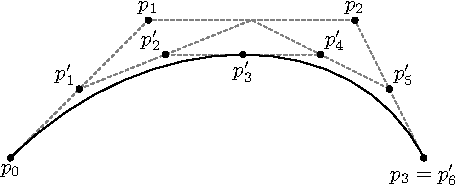
\includegraphics{subdivision}
% 	     \caption{A Figure}
% 	 \label{subd}
% 	\end{figure}

% \clearpage %% starts a new page and stops trying to place floats such as tables and figures

% \section{More Figure Stuff}
% You can also scale and rotate figures.
%  	\begin{figure}[h!]
	   
% 	       \centering
% 	    % DO NOT ADD A FILENAME EXTENSION TO THE GRAPHIC FILE
% 	    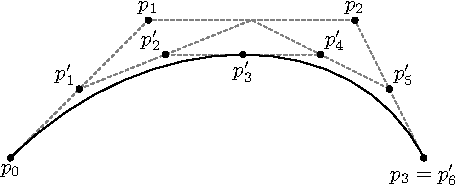
\includegraphics[scale=0.5,angle=180]{subdivision}
% 	    % if your figure shows up not where you want it, it may just be too big to fit. You can use the scale argument to shrink it, e.g. scale=0.85 is 85 percent of the original size. 
% 	     \caption{A Smaller Figure, Flipped Upside Down}
% 	 \label{subd2}
% 	\end{figure}

% \section{Even More Figure Stuff}
% With some clever work you can crop a figure, which is handy if (for instance) your EPS or PDF is a little graphic on a whole sheet of paper. The viewport arguments are the lower-left and upper-right coordinates for the area you want to crop.

%  	\begin{figure}[h!]
% 	    	       \centering
% 	    % DO NOT ADD A FILENAME EXTENSION TO THE GRAPHIC FILE
% 	   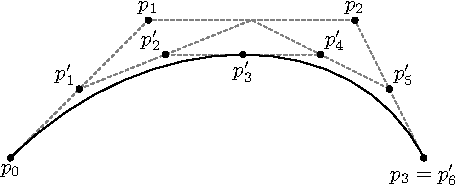
\includegraphics[clip=true, viewport=.0in .0in 1in 1in]{subdivision}
% 	    \caption{A Cropped Figure}
% 	 \label{subd3}
% 	\end{figure}
	
%       \subsection{Common Modifications}
   %    The following figure features the more popular changes thesis students want to their figures. This information is also on the web at \url{web.reed.edu/cis/help/latex/graphics.html}.
   %  %\renewcommand{\thefigure}{0.\arabic{figure}} 	% Renumbers the figure to the type 0.x
   %  %\addtocounter{figure}{4} 						% starts the figure numbering at 4
   %  \begin{figure}[htbp]
   %  \begin{center}
   % 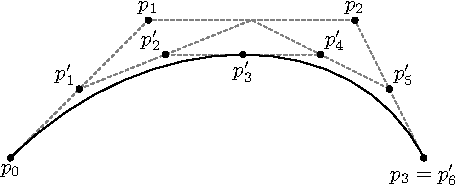
\includegraphics[scale=0.5]{subdivision}
   %  \caption[Subdivision of arc segments]{\footnotesize{Subdivision of arc segments. You can see that $ p_3 = p_6^\prime$.}} %the special ToC caption is in square brackets. The \footnotesize makes the figure caption smaller
   %  \label{barplot}
   %  \end{center}
   %  \end{figure} 

% \chapter*{Conclusion}
%          \addcontentsline{toc}{chapter}{Conclusion}
% 	\chaptermark{Conclusion}
% 	\markboth{Conclusion}{Conclusion}
% 	\setcounter{chapter}{4}
% 	\setcounter{section}{0}
	
% Here's a conclusion, demonstrating the use of all that manual incrementing and table of contents adding that has to happen if you use the starred form of the chapter command. The deal is, the chapter command in \LaTeX\ does a lot of things: it increments the chapter counter, it resets the section counter to zero, it puts the name of the chapter into the table of contents and the running headers, and probably some other stuff. 

% So, if you remove all that stuff because you don't like it to say ``Chapter 4: Conclusion'', then you have to manually add all the things \LaTeX\ would normally do for you. Maybe someday we'll write a new chapter macro that doesn't add ``Chapter X'' to the beginning of every chapter title.

% \section{More info}
% And here's some other random info: the first paragraph after a chapter title or section head \emph{shouldn't be} indented, because indents are to tell the reader that you're starting a new paragraph. Since that's obvious after a chapter or section title, proper typesetting doesn't add an indent there. 


%If you feel it necessary to include an appendix, it goes here.
%This is where endnotes are supposed to go, if you have them.
%I have no idea how endnotes work with LaTeX.

  \backmatter % backmatter makes the index and bibliography appear properly in the t.o.c...

% if you're using bibtex, the next line forces every entry in the bibtex file to be included
% in your bibliography, regardless of whether or not you've cited it in the thesis.
    \nocite{*}

% Rename my bibliography to be called "Works Cited" and not "References" or ``Bibliography''
\renewcommand{\bibname}{Works Cited}

%    \bibliographystyle{bsts/mla-good} % there are a variety of styles available; 
%  \bibliographystyle{plainnat}
% replace ``plainnat'' with the style of choice. You can refer to files in the bsts or APA 
% subfolder, e.g. 
 \bibliographystyle{APA/apa-good}  % or
 \bibliography{thesis}
 % Comment the above two lines and uncomment the next line to use biblatex-chicago.
 %\printbibliography[heading=bibintoc]

% Finally, an index would go here... but it is also optional.
\end{document}
